\chapter{Development of the FPGA firmware for the SFH}\label{cha:development}
\section{Overview of the firmware} 
The firmware developed in this thesis for the three Artix-7 FPGAs, located on the iFTDC as described in Section \ref{sec:iFTDC}, must perform several functionalities.
The main tasks of the firmware are to configure the Citiroc1A ASIC, explained in Section \ref{sec:configuration},
 communicaton with the controlling coputer via ethernet and the IPBUS protocol and a provisional readout of the time triggerd data from the Citiroc1A ASIC.
\newline
The fimrmware is written in VHSIC Hardware Description Language (VHDL) and is synthesized and implemented using the Xilinx Vivado Design Suite.
Several IP-cores, provided by Xilinx, are used to simplfy the development of the firmware for several task like the implementation of  the memory.
\subsection{The IPBUS protocol}
The IPBUS protocol used for the communication between the FPGA and the controlling computer is a simple protocol for controlling IP-aware hardware devices with a 32 bit read and write bus using UDP as the transport protocol.\autocite{IPBUS_article}
\newline
The IPBUS protocol defines a read and write command enabling successful write and read operations of a 32 bit register, with a 32 bit address in the FPGA.    
\newline
The commands can be issued on the controling computer with the $\mu$HAL library, which allowes the user to issue read and write commands with a python script and an XML file defining the address of the registers.\autocite{IPBUS_article}
\newline
The address space inside the FPGA is defined in the firmware. The address space is divided into seprate address spaces for each of the slaves by the leading bits of the address.
For some slaves, the address space is further divided into subspaces for the different registers of the slave.


\subsection{The firmware structure}
\begin{tikzpicture}[node distance=2cm]

    % Top-level module
    \node (top) [block] {Top-Level Module};
    
    % Submodules
    \node (wrapper) [block, below =2.5cm and 0.5cm of top] {Wrapper Module};
    \node (sync) [block, below left  =0.5 cm and 0.5cm of top] {Synchronizer Module};
    
    % Wrapper components
    \node (ipbus) [block, below left=1.5cm and 2.5cm of wrapper] {IPBus Protocol Logic};
    \node (addr) [block, below=1.5cm of wrapper] {Address Decoding Logic};
    \node (slaves) [block, below right=1.5cm and 1.5cm of wrapper] {Slave Module};
    
    
    % Slave module components
    \node(Citiroc1A 1)[block, below left=2cm and 5cm of slaves] {Citiroc1A ASIC 1};
    \node(Citiroc1A 2)[block, below left  =2cm and -1.5cm of slaves] {Citiroc1A ASIC 2};
    %ASIC 1
    \node (config1) [block, below left =3.5cm and -1cm of Citiroc1A 1 ] {Citiroc1A Interface};
    \node (hitcounters1) [ block, below right =3.5cm and -1cm of Citiroc1A 1] {Hit Counters (32)};
    %ASIC 2
    \node (config2) [block,  below right =1.5cm and -1cm of Citiroc1A 2] {Citiroc1A Interface};
    \node (hitcounters2) [ block,below left = 1.5cm and -1cm    of Citiroc1A 2] {Hit Counters (32)};
    %config1
    \node (confi1) [block, below left=1.5cm and -1cm of config1 ] {Configuration SM};
    \node (verif1) [block, below right =1.5cm and -1cm of config1] {Verification SM};
    %config1
    \node (confi2) [block, below left=2.5cm and 0cm of config2 ] {Configuration SM};
    \node (verif2) [block, below  =2.5cm and -1cm of config2] {Verification SM};
    % Arrows
    \draw [arrow] (top) -- (wrapper);
    \draw [arrow] (top) -- (sync);
    \draw [arrow] (wrapper) -- (ipbus);
    \draw [arrow] (wrapper) -- (addr);
    \draw [arrow] (wrapper) -- (slaves);
    \draw [arrow] (slaves) -- (Citiroc1A 1);
    \draw [arrow] (slaves) -- (Citiroc1A 2);
    \draw [arrow] (Citiroc1A 1) -- (config1);
    \draw [arrow] (Citiroc1A 1) -- (hitcounters1);
    \draw [arrow] (Citiroc1A 2) -- (config2);
    \draw [arrow] (Citiroc1A 2) -- (hitcounters2);
    \draw [arrow] (config1) -- (confi1);
    \draw [arrow] (config1) -- (verif1);
    \draw [arrow] (config2) -- (confi2);
    \draw [arrow] (config2) -- (verif2);
    
        
    \end{tikzpicture}
The firmware has a hierarchical structure. In this section, I will describe the structure of the relevant components of the firmware.
\newline
The top level modul of the firmware contains the outgoing and incoming signals of the FPGA.
\newline
The top level modul instantiates a wrapper modul for the IPBUS protocol and the slave entities and a synchronizer modul for the incoming time triggerd Citiroc1A signals. 
\newline
The wrapper modul  contains the IPBUS protocol logic and the address decoding logic as well as a modul containing the slaves.
\newline
The slave modul contains several slaves for the different tasks of the firmware. For each of the Citiroc1A ASICs, a slave is instantiated for the configuration and verification of the ASIC, along with
32 hitcounters for the 32 channels of the Citiroc1A ASIC. 



\section{Configuration of the Citiroc1A ASIC}

The configuration of the slow control and probe registers of the Citiroc1A ASIC,
 along with the verification of this configuration, is handled by two finite state machines. Both state machines each control a random access memory (RAM) with a depth of 64 addresses, where each address stores 32 bits of data.
The state machiens in turn are controled by the status and control register, which can be written by the controlling computer via the ipbus protocol.
\subsection{Status and control register}

\subsection{Configuration state machine}
\begin{figure}[H]
    \centering
    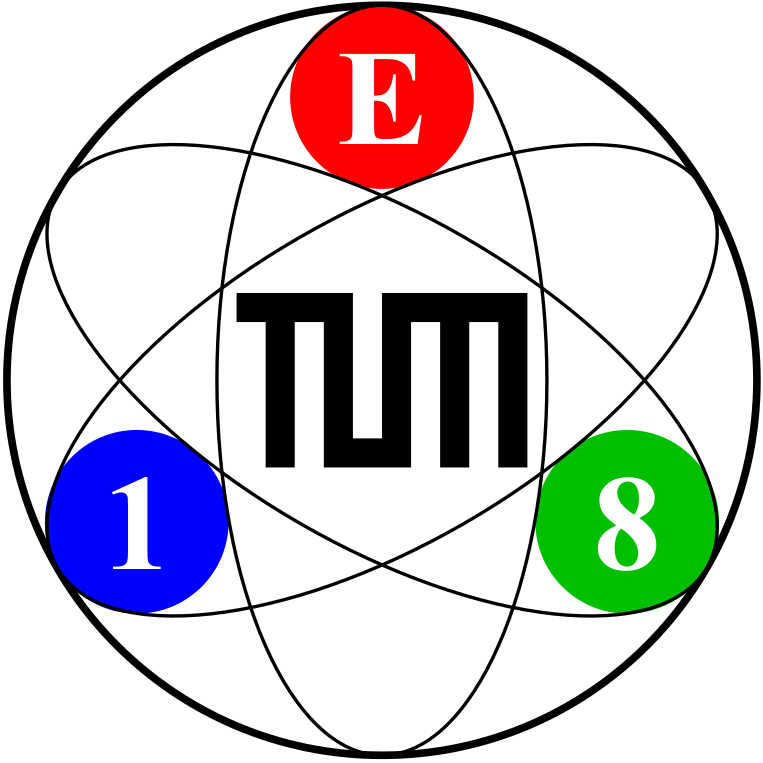
\includegraphics[width=\textwidth]{E18Logo.png}%{CONFIGSMALLdiagramfarbe3000.png}
    \caption{Finite state machine for configuring the Citiroc1A ASIC.
    States associated with the same processes are highlighted using the same color.}
    \label{fig:Configuration_state_machine}
\end{figure}
\subsection{Verification state machine}
\begin{figure}[H]
    \centering
    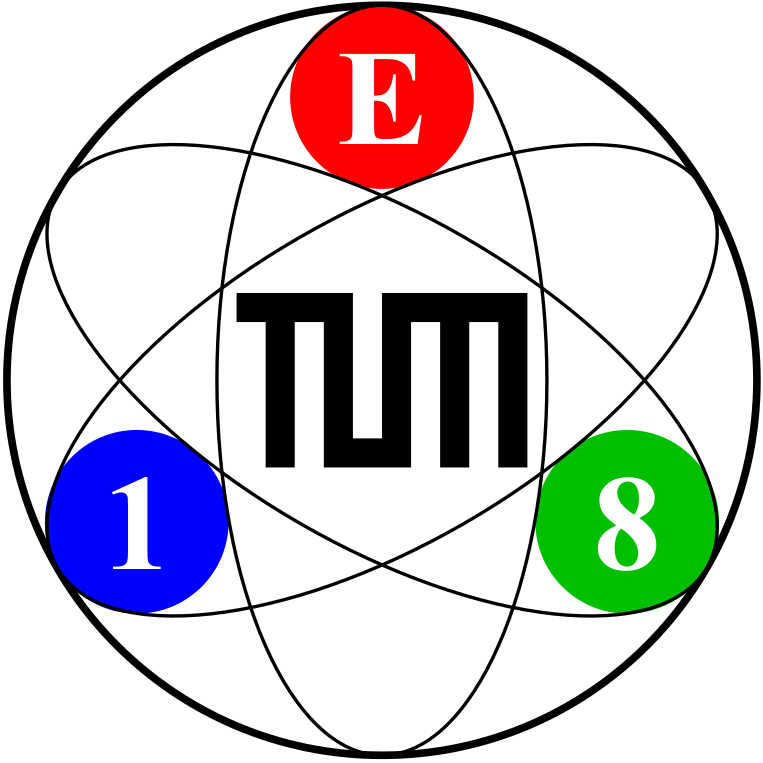
\includegraphics[width=\textwidth]{E18Logo.png}%{smallVerifacationdiagrammodfarbe.png}
    \caption{Finite state machine for verifying the configuration of the Citiroc1A ASIC.
    States belonging to the same processes are represented with the same color.}
    \label{fig:Verification_state_machine}
\end{figure}
